%% =============================================================
%%  ANLP Assignment 1 -- Report
%%  Transformer-based Cipher Decryption: Ablation Study (C1-C5)
%%  Compile: pdflatex report.tex  (run twice for cross-references)
%% =============================================================
\documentclass[12pt,a4paper]{article}

%% --- Packages ---
\usepackage[margin=1in]{geometry}
\usepackage{mathptmx}           % Times New Roman (text + math)
\usepackage[T1]{fontenc}
\usepackage[utf8]{inputenc}
\usepackage{microtype}
\usepackage{graphicx}
\usepackage{booktabs}
\usepackage{multirow}
\usepackage{array}
\usepackage{tabularx}
\usepackage{float}
\usepackage{caption}
\usepackage{subcaption}
\usepackage{amsmath}
\usepackage{amssymb}
\usepackage[hidelinks,colorlinks=true,linkcolor=blue,urlcolor=blue,citecolor=blue]{hyperref}
\usepackage{url}
\usepackage{xurl}
\usepackage{enumitem}
\usepackage{parskip}
\usepackage[numbers,sort&compress]{natbib}

%% --- Layout ---
\usepackage{titlesec}
\setlength{\parskip}{3pt}
\setlength{\parindent}{0pt}
\captionsetup{font=small, labelfont=bf}
\titlespacing*{\section}{0pt}{7pt}{3pt}
\titlespacing*{\subsection}{0pt}{5pt}{2pt}
\renewcommand{\arraystretch}{0.88}

\newcommand{\modelname}[1]{\textbf{\texttt{#1}}}

\begin{document}

%% --- Title ---
\begin{center}
    {\Large\bfseries ANLP Assignment 1}\\[4pt]
    {\normalsize Yash More, 2024114004}
\end{center}

\vspace{4pt}
\hrule
\vspace{4pt}

%% ============================================================
\section*{Abstract}

We treat cipher decryption as a sequence-to-sequence translation problem and train a Transformer from scratch to translate an encrypted stream into the original English text. The cipher encodes every plaintext character into a fixed 8-bit code, but the mapping is not a fixed lookup table: the same 8-bit block can decode to different characters depending on where it sits in the sequence, so the model has to use position and context, not memorization, to invert it. Our baseline (C1) already represents the ciphertext at the byte level (each 8-bit block as a single integer token) and only applies BPE to the plaintext it outputs. Starting from this baseline, we ablate four components one at a time: Rotary Positional Encoding (C2), Grouped-Query Attention (C3), RMSNorm (C4), and a fully token-free, byte-level architecture (C5, following the Byte Latent Transformer) that drops BPE entirely and processes the ciphertext as a raw bit stream. All five configurations are evaluated on the full held-out test set (4,782 examples) with greedy decoding. C5 gives by far the best reconstruction quality, reaching 99.95\% bit accuracy and a mean Levenshtein distance of 0.06, while also being the smallest model by parameter count and, once every configuration is compared on equal hardware (a single GPU each), the fastest per epoch as well. Among the tokenized models (C1-C4), every single ablated component (RoPE, GQA, or RMSNorm) improves on the plain C1 baseline, with RoPE (C2) the strongest of the three.

%% ============================================================
\section{Introduction}

The task is character-level decryption framed as sequence-to-sequence translation. Given a line of ciphertext $X$, the model must produce the corresponding plaintext line $Y$. Our first step, before touching any architecture, was to look at the data, since the design of the whole pipeline depends on what kind of cipher this is.

Analyzing \texttt{brown\_plain.txt} and \texttt{brown\_cipher.txt} (full findings in \texttt{analysis.md}) showed three things that shaped every later decision. First, the cipher is a fixed-length encoding: every plaintext character maps to exactly 8 bits. Second, newlines are not encrypted; they are kept as literal line breaks, which is why we process the data line by line rather than as one continuous stream. Third, and most importantly, the cipher is not a simple substitution: the same 8-bit block decodes to different characters in different places (117 such sequences map to more than one character), which rules out a static lookup table and tells us the cipher is context- or position-dependent, similar in spirit to a polyalphabetic or stream cipher. This is why positional encoding is arguably the most important design choice in the whole assignment, and why C2 (RoPE) and C5 (offset-aware, byte-level positions) are the two ablations we cared about most.

We train five configurations (C1-C5) on the Brown-corpus-derived cipher dataset (5,001 lines) using an Encoder-Decoder Transformer built from scratch (attention, normalization, and positional encoding are our own implementations, not framework layers), on NVIDIA RTX 2080 Ti GPUs with mixed precision. Every final run in this report trained on a single GPU; an earlier version of C1 trained on 4 GPUs with DDP, and we retrained it on a single GPU once we realized the mismatch made its speed and memory numbers incomparable to C2-C5. All reported metrics use greedy decoding on the full held-out test split (4,782 examples), not a small subsample.

%% ============================================================
\section{Experimental Setup}

\textbf{Hardware \& data.} All five final runs trained on a single RTX 2080 Ti GPU (11 GB VRAM) on the Ada cluster, using \texttt{torch.autocast} FP16, gradient accumulation, and pinned-memory dataloaders. The base dataset has 5,001 aligned (ciphertext, plaintext) lines. To fight overfitting on this small corpus, every configuration trains on a sliding-window chunked version of the data (64-character windows with absolute byte-offset tracking so the positional encoding stays correct), expanding the training split to 39,683 examples (val: 4,685, test: 4,782), identically for all five configurations (Section 3 explains why).

\textbf{Tokenization.} Worth stating precisely, since it is easy to get wrong: in C1-C4, the ciphertext is \emph{already} byte-level, not BPE. Each 8-bit block is grouped into a single integer token (0-255 plus 3 special tokens, vocabulary 259), and BPE is applied only to the plaintext the decoder produces (vocabulary 5,000). C5 removes BPE from the plaintext side too: it reads the ciphertext as a raw bit stream, one token per `0`/`1` character, with a lightweight local encoder grouping every 8 bits into a patch internally, and writes plaintext as raw UTF-8 bytes. Table~\ref{tab:hparams} lists the shared hyperparameters, taken directly from the final training configuration (verified against \texttt{src/train.py} and the logged parameter counts in \texttt{outputs/c1.log}-\texttt{c5.log}, not our earlier exploratory notes, which used different values before the Section 3 tokenization fix).

\begin{table}[H]
\centering
\small
\begin{tabularx}{\linewidth}{llX}
\toprule
\textbf{Hyperparameter} & \textbf{Value} & \textbf{Notes} \\
\midrule
\texttt{d\_model} / \texttt{d\_ff} & 256 / 1024 & $4\times$ expansion \\
\texttt{n\_heads} & 8 & $d_k=32$; $n_{\text{kv\_heads}}=2$ for C3 \\
\texttt{num\_layers} & 6 enc + 6 dec & \\
\texttt{chunk\_size} & 64 & Effective sequence length is \texttt{chunk\_size}+2 \\
\texttt{plaintext BPE vocab} & 5000 & C1-C4 decoder output only, unused in C5 \\
\texttt{cipher vocab} & 259 & Byte ints (C1-C4) or raw bits (C5), + specials \\
\texttt{learning\_rate} & $1.5\times10^{-3}$ & Linear warmup (5\%) + cosine decay \\
\texttt{dropout} / \texttt{wd} / \texttt{ls} & 0.3 / 0.05 / 0.2 & Weight decay, label smoothing \\
\texttt{batch\_size} & 20/GPU, 1 GPU, 3 accum & Effective batch 60 (same for all five) \\
\bottomrule
\end{tabularx}
\caption{Architecture and optimization hyperparameters shared by all five final runs (only the ablated component differs). Cross-checked against \texttt{src/train.py} defaults and the parameter counts logged for each run.}
\label{tab:hparams}
\end{table}

%% ============================================================
\section{How We Got Here: The Hyperparameter Search}

The configuration in Table~\ref{tab:hparams} did not come from a single design pass; it is the result of a back-and-forth between what the cipher analysis said should work and what actually trained well.

\textbf{Capacity and tokenization.} Early on, with a pipeline that applied BPE directly to the raw ciphertext bit-string, a controlled sweep across model sizes (Figure~\ref{fig:capacity_sweep}) suggested the cipher needed a large model to compensate for badly-behaved BPE merges over raw bits: the two \texttt{d\_model}=512 runs (51M and 37M parameters) kept dropping well past step 100, while the two \texttt{d\_model}=256 runs (14.9M parameters, and a 13M-parameter run on an 8-bit representation) plateaued far higher over the same steps. But the real problem was upstream: BPE merges whatever bit patterns occur most frequently with no notion of where an 8-bit character boundary starts or ends, so applying it to the `0`/`1` string was destroying the one signal (absolute position within a byte) the model needed most. We fixed this by converting each 8-bit chunk to its integer value (0-255) and feeding that directly as a token, with no BPE on the cipher side; this byte-grouped representation is what all of C1-C4 use. Separately, a sequence-length experiment (Figure~\ref{fig:seqlen_sweep}) showed that shrinking the sequence length made the loss worse, not better as expected. In the seq\_len=64 and seq\_len=256 runs, every line longer than that limit was simply truncated, and this was before the chunking fix described below, so training saw only the original 5,001 lines cut down to a handful of tokens each; a model this size should have been able to essentially memorize a training set that small, yet the loss barely moved. The cause was not capacity but learning rate: these runs used $1\times10^{-4}$, and our LR scheduler shrank it even further as training went on, so the effective step size collapsed before the model could fit even this small a training set. We then tried several higher rates ($1\times10^{-3}$, $3\times10^{-3}$, $1.5\times10^{-3}$) and settled on $1.5\times10^{-3}$, which fixed convergence immediately.

\begin{figure}[H]
    \centering
    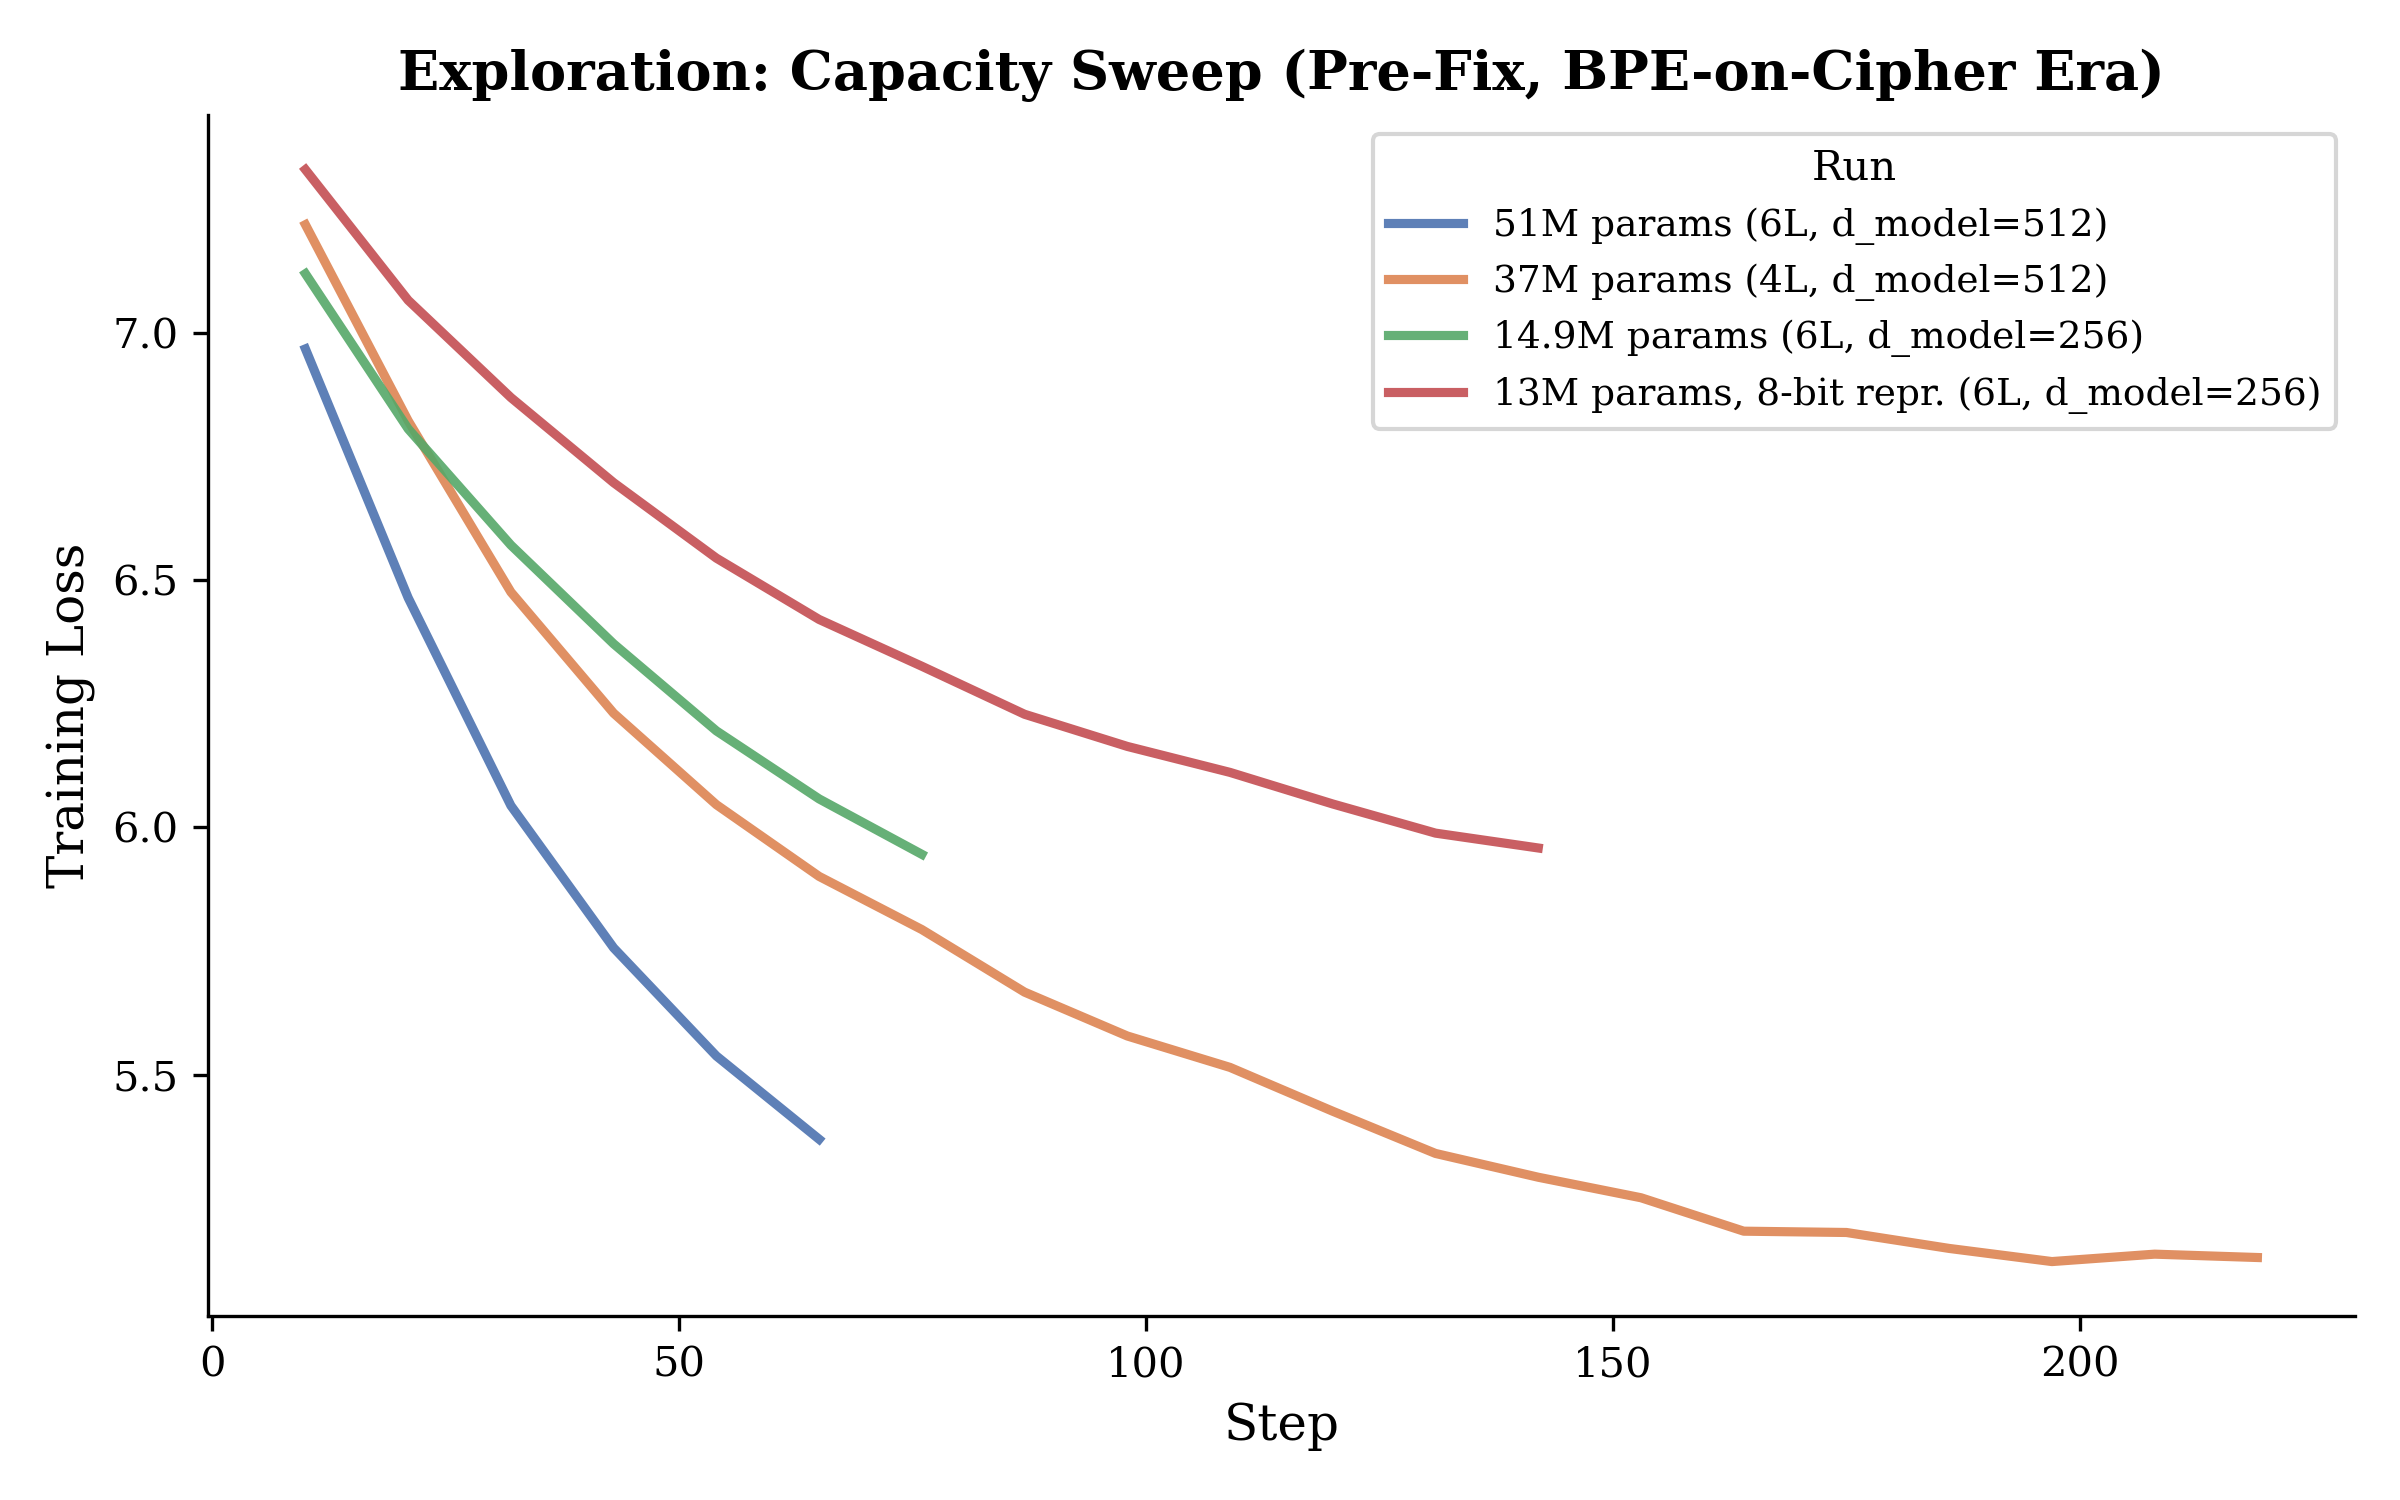
\includegraphics[width=0.75\linewidth]{outputs/exploration_capacity_sweep.png}
    \caption{Training loss vs.\ step for the pre-fix model-capacity sweep (BPE applied directly to the cipher bit-string).}
    \label{fig:capacity_sweep}
\end{figure}

\begin{figure}[H]
    \centering
    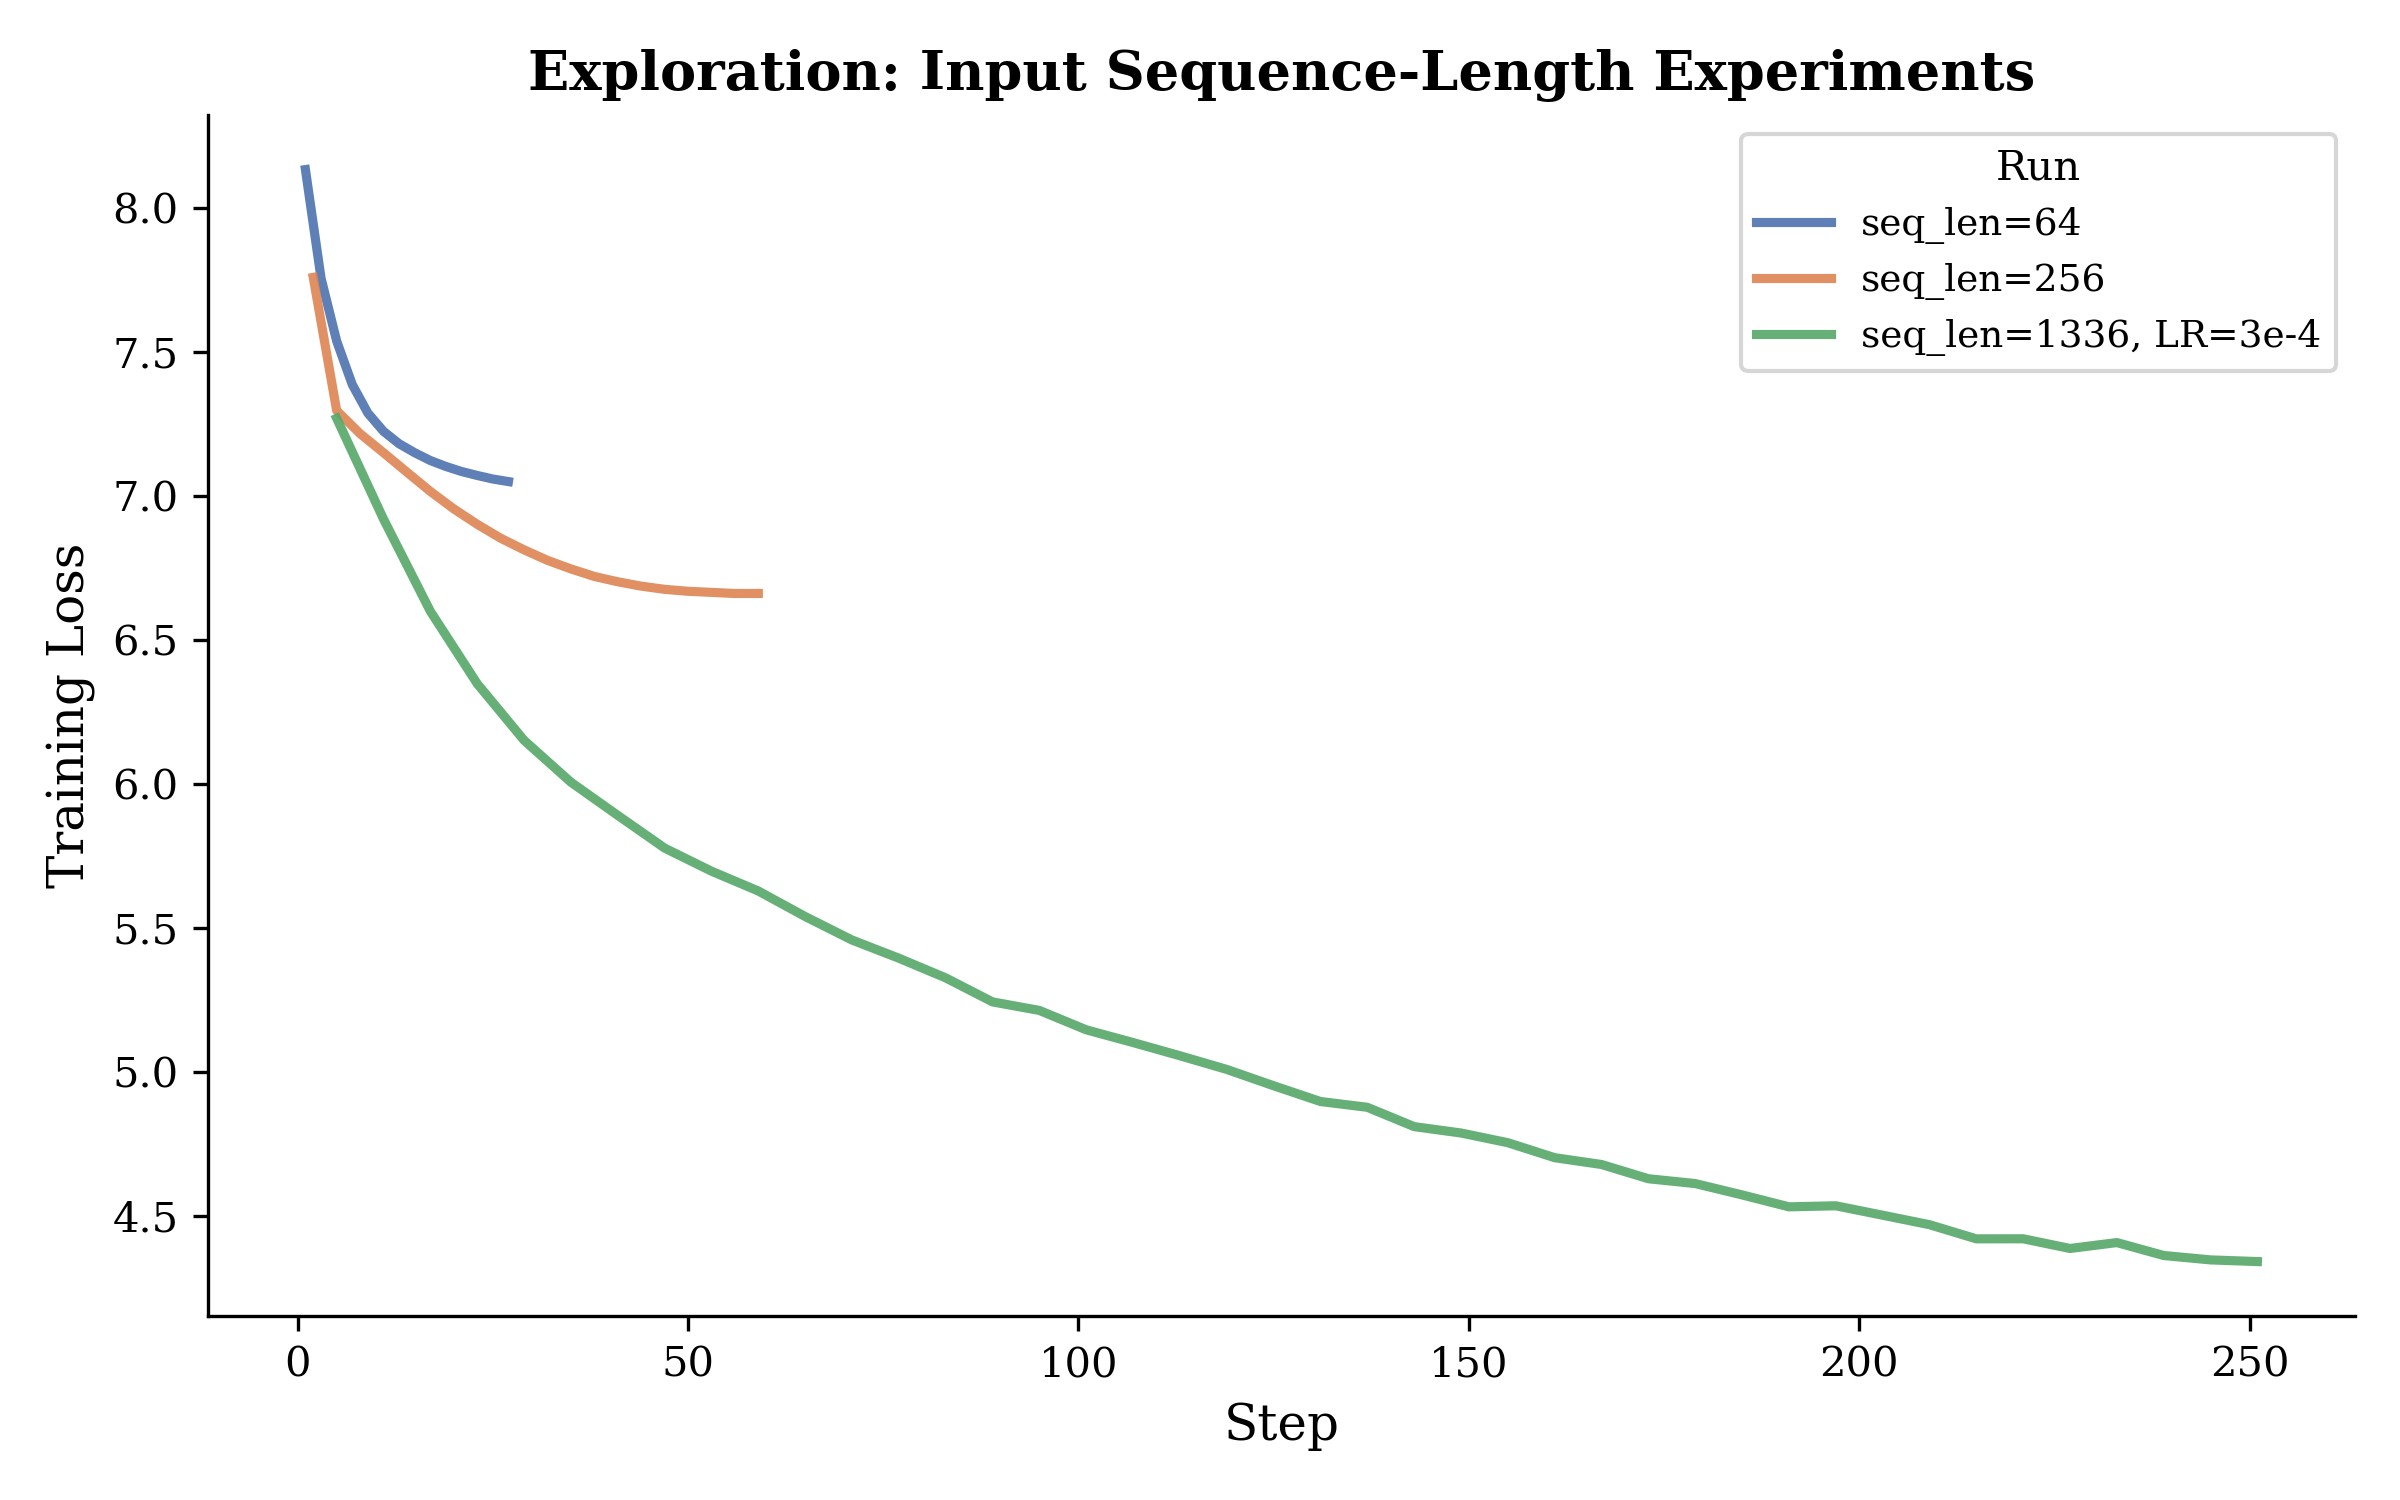
\includegraphics[width=0.75\linewidth]{outputs/exploration_seqlen_sweep.png}
    \caption{Training loss vs.\ step for the input sequence-length experiments.}
    \label{fig:seqlen_sweep}
\end{figure}

\textbf{Chunking, then a smaller model than expected.} With byte-grouped cipher tokens in place, the model overfit almost immediately on our $\sim$4,000-line dataset. Figure~\ref{fig:lr_epoch_sweep} shows this transition: the seq\_len=512 learning-rate/epoch-budget sweep (blue/orange/green) and the two early no-BPE-cipher runs (red/purple) all converge along a similar trajectory over a few hundred steps, well short of where the final configurations end up. Fixed-size, non-overlapping 64-character chunking (each chunk tagged with its absolute byte offset so the positional encoding stays correct) grew the training set to nearly 40,000 examples and pushed overfitting much later into training; we then re-tuned dropout, weight decay, and label smoothing (0.3/0.05/0.2 gave the best balance). Once the cipher tokenizer no longer needed internal correction, the earlier capacity wall mostly disappeared: the final C1 uses \texttt{d\_model}=256, the same size that plateaued badly in the pre-fix sweep, and comfortably beats what the sweep saw even at \texttt{d\_model}=512. Most of the capacity the earlier sweep seemed to need was compensating for a broken cipher tokenizer, not the task itself.

\begin{figure}[H]
    \centering
    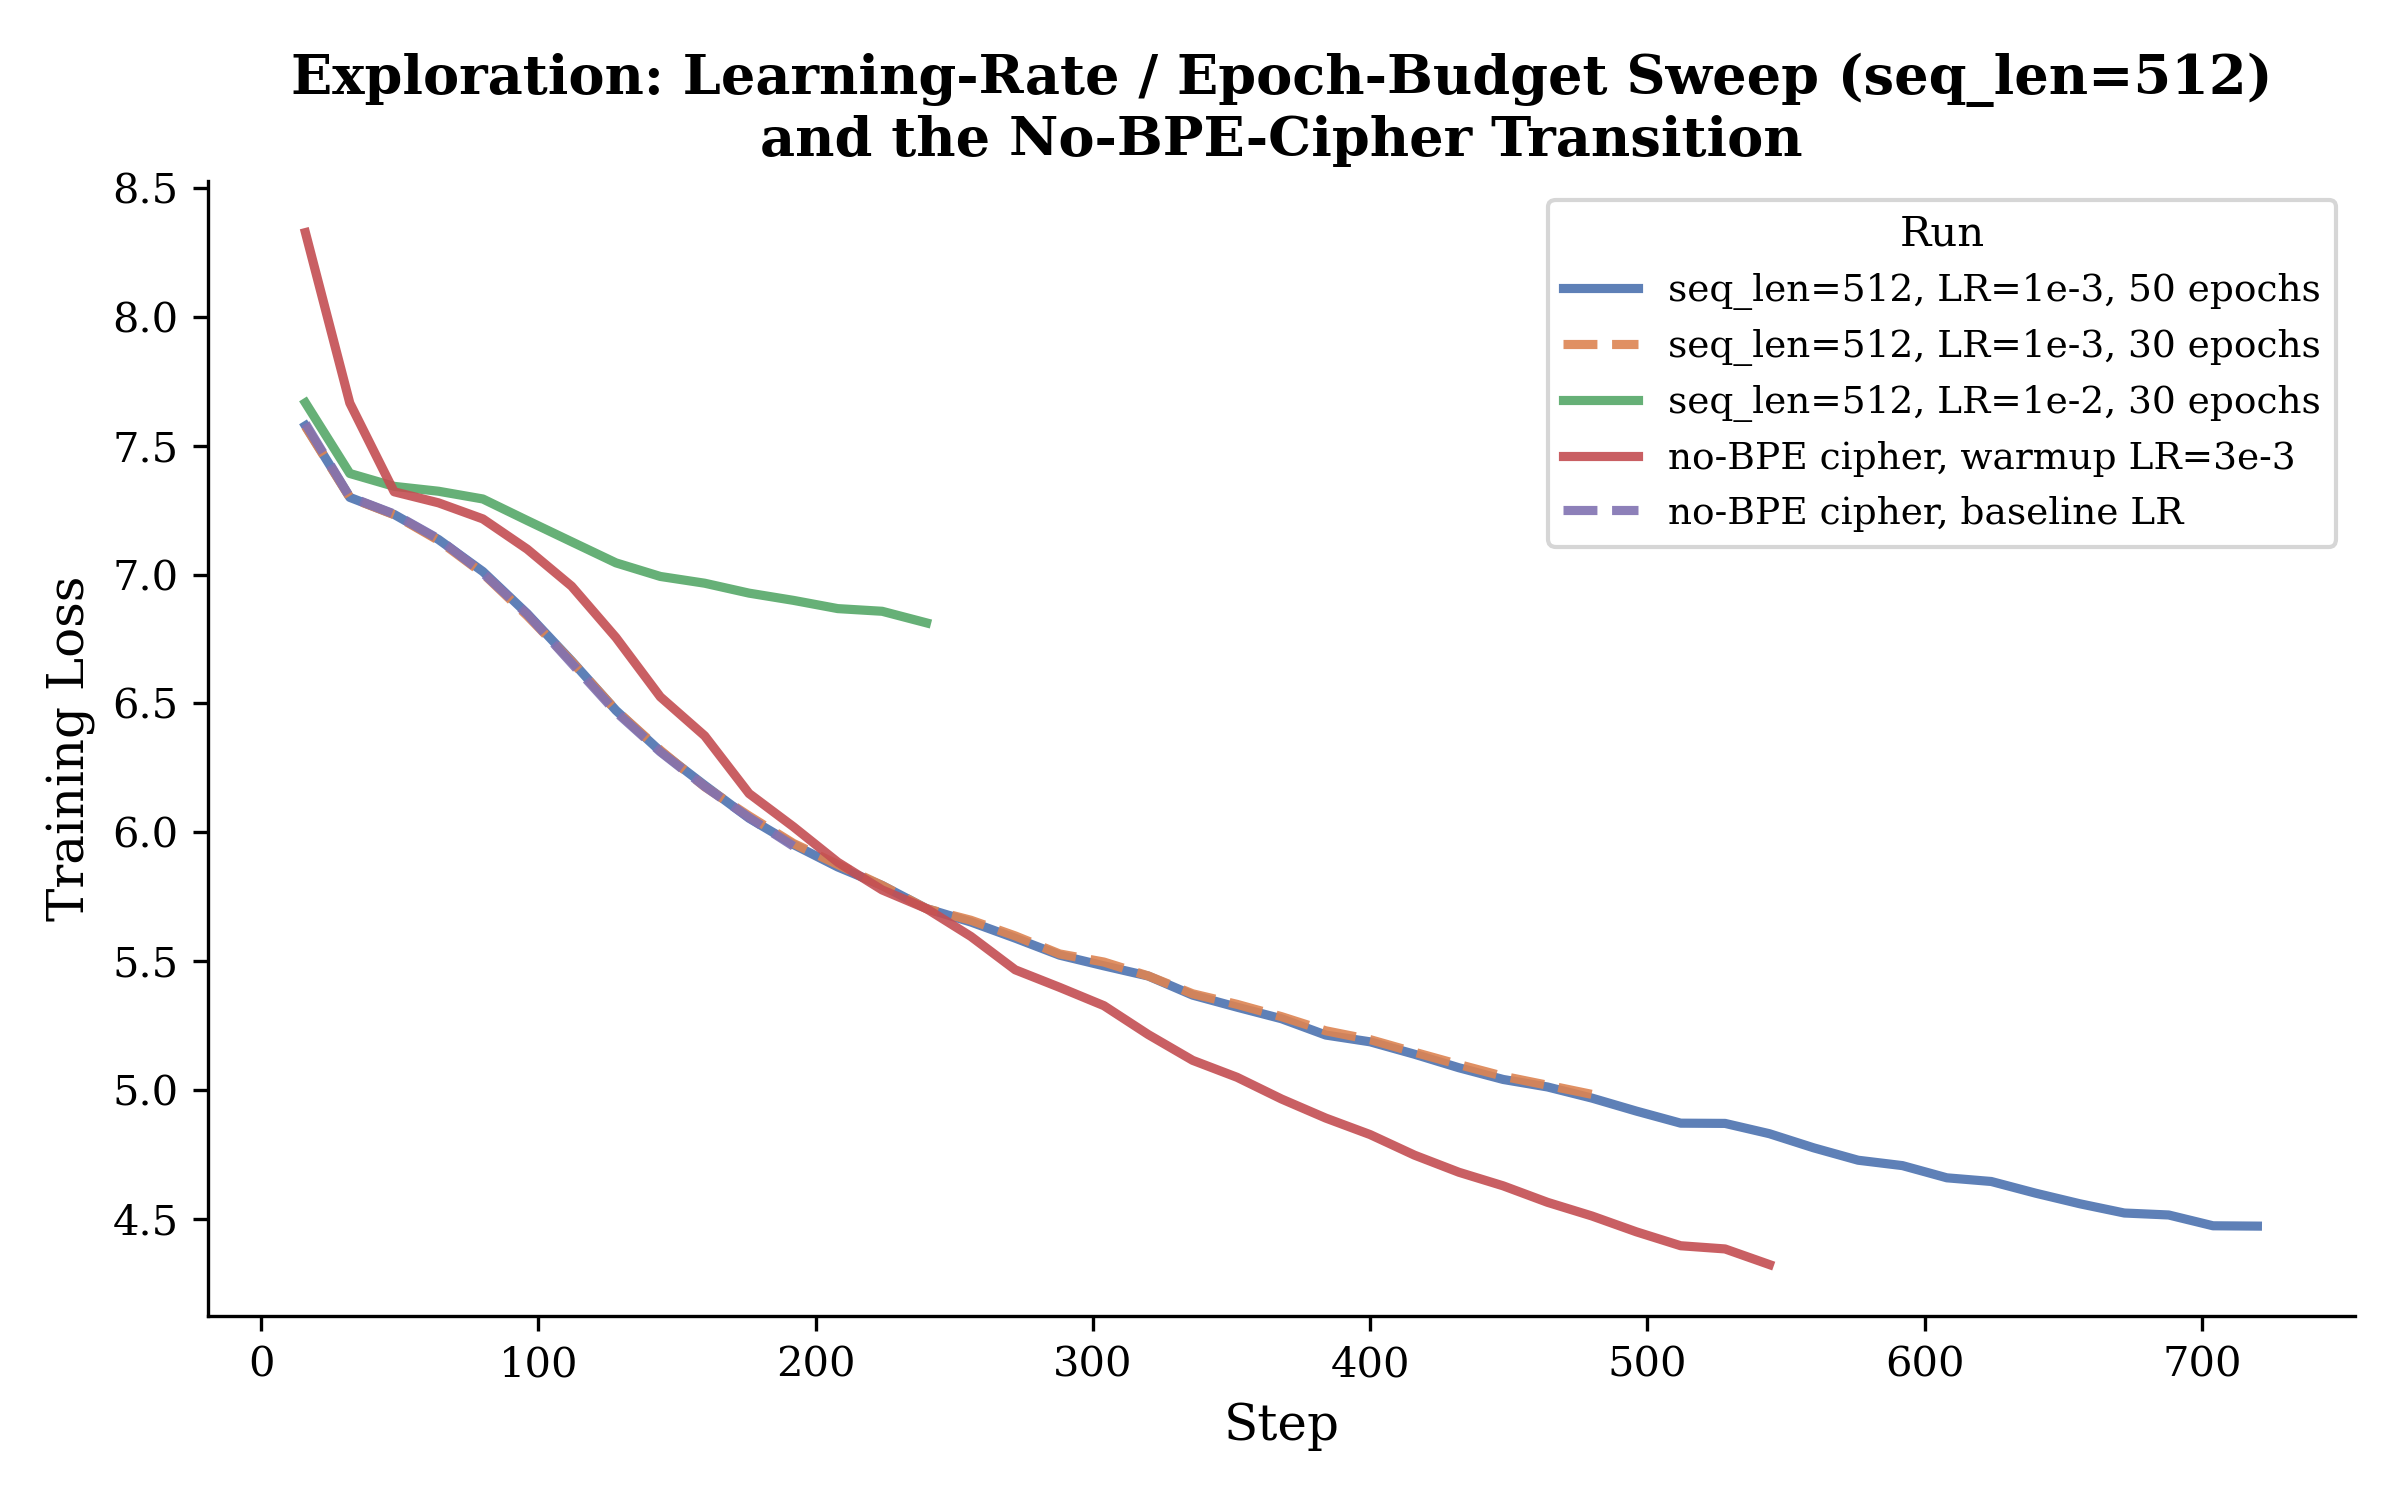
\includegraphics[width=0.75\linewidth]{outputs/exploration_lr_epoch_sweep.png}
    \caption{Training loss vs.\ step for the seq\_len=512 learning-rate/epoch-budget sweep and the early no-BPE-cipher runs, before chunking was introduced.}
    \label{fig:lr_epoch_sweep}
\end{figure}

\textbf{A hardware fairness fix, late in the project.} Our first full C1 run trained on 4 GPUs with DDP, while C2-C5 each trained on a single GPU; we did not realize until writing this report that the mismatch made the Section 6 comparison meaningless, so we retrained C1 on a single GPU with every other hyperparameter unchanged and use that run throughout. One caveat: the learning rate was tuned against C1's original 4-GPU effective batch size of 240, and the retrain reuses it against an effective batch size of 60, the regime C2-C5 already trained under without separate tuning. The single-GPU C1 converges to a visibly worse best validation loss than the original 4-GPU run (0.234 vs.\ roughly 0.12-0.14 per epoch) and stops earliest of all five configurations, at epoch 40. This does not invalidate the comparison, since C2-C4 share the same untuned rate and batch size, but Section 5's ablation results should be read as comparisons under one shared, not per-configuration-optimal, training regime. The single-GPU C1 curve itself is shown alongside C2-C5 in Figure~\ref{fig:val_loss_final}, not repeated here.

%% ============================================================
\section{Model Configurations}

Each of C2-C5 changes exactly one component relative to C1, so any difference in results can be attributed to that single change.

\begin{table}[H]
\centering
\small
\begin{tabularx}{\linewidth}{llX}
\toprule
\textbf{Config} & \textbf{Change from C1} & \textbf{Description} \\
\midrule
\modelname{C1} & Baseline & Sinusoidal absolute PE, standard multi-head attention, Pre-LayerNorm; cipher input as byte-grouped integer tokens, plaintext output BPE-tokenized \\
\modelname{C2} & +RoPE \cite{su2024roformer} & Sinusoidal PE replaced by Rotary Position Embeddings inside attention \\
\modelname{C3} & +GQA \cite{ainslie2023gqa} & Grouped-Query Attention, $n_{\text{kv\_heads}}=2$ instead of 8 \\
\modelname{C4} & +RMSNorm \cite{zhang2019rmsnorm} & LayerNorm replaced by RMSNorm \\
\modelname{C5} & BLT-style \cite{pagnoni2024blt} & No BPE on either side; cipher read as a raw bit stream (one token per `0`/`1`) grouped into 8-bit patches by a local encoder, plaintext written as raw UTF-8 bytes \\
\bottomrule
\end{tabularx}
\caption{Architectural changes for each configuration relative to the C1 baseline.}
\end{table}

%% ============================================================
\section{Results}

\subsection{Quantitative Metrics}

Table~\ref{tab:results} reports every metric on the \emph{full} held-out test split (4,782 examples) using greedy decoding. BLEU and ROUGE are word-level n-gram metrics, so we only report them for the tokenized models (C1-C4); they are not meaningful for C5, which never groups characters into subword units. An earlier pass at this evaluation used only 5 test examples due to a leftover debugging shortcut in our dataloader construction; we caught this, fixed the dataloader, and re-evaluated every checkpoint on the complete test set, so every number below is statistically meaningful rather than an artifact of a 5-sample sample.

\begin{table}[H]
\centering
\small
\begin{tabular}{lrrrrr}
\toprule
\textbf{Metric} & \textbf{C1} & \textbf{C2} & \textbf{C3} & \textbf{C4} & \textbf{C5 (BLT)} \\
\midrule
Parameters      & 13.69M & 13.69M & 11.91M & 13.68M & \textbf{7.11M} \\
val\_loss        & 0.2047 & \underline{0.1093} & 0.1894 & 0.1927 & \textbf{0.0801} \\
Bit Accuracy    & 84.56\% & \underline{91.50\%} & 87.40\% & 87.64\% & \textbf{99.95\%} \\
Seq Accuracy    & 68.83\% & \underline{80.19\%} & 72.90\% & 73.87\% & \textbf{97.00\%} \\
Levenshtein     & 2.83 & \underline{1.74} & 2.43 & 2.35 & \textbf{0.06} \\
BLEU            & 0.9359 & \textbf{0.9606} & 0.9458 & 0.9460 & N/A \\
ROUGE-1         & 0.9626 & \textbf{0.9770} & 0.9683 & 0.9689 & N/A \\
ROUGE-2         & 0.9455 & \textbf{0.9665} & 0.9540 & 0.9543 & N/A \\
ROUGE-L         & 0.9626 & \textbf{0.9770} & 0.9682 & 0.9688 & N/A \\
\bottomrule
\end{tabular}
\caption{Final test-set evaluation metrics on the full 4,782-example test split, greedy decoding. Bold marks the best value in each row overall; underline marks the best among the tokenized models (C1-C4) where C5 is not comparable (BLEU/ROUGE) or is trivially best by construction. Parameter counts are from the trained checkpoints.}
\label{tab:results}
\end{table}

\subsection{Convergence}

Figure~\ref{fig:val_loss_final} plots validation loss over training for all five configurations. C2, C3, and C4 all run close to the full 50 epochs. C5 triggers early stopping at epoch 46, after its validation loss had already dropped well below every other configuration. C1 stops earliest of all, at epoch 40, and its curve is visibly different in shape: it drops fastest in the first 5-10 epochs, but plateaus by around epoch 10 while C2, C3, and C4 are still well above it, and those three eventually cross below C1 and keep improving. This pattern is consistent with the effective-batch-size caveat noted in Section 3: C1's single-GPU retrain converges quickly under a learning rate tuned for a larger batch, then stalls, whereas the other configurations (already trained at this smaller effective batch size from the start) continue to improve for longer.

\begin{figure}[H]
    \centering
    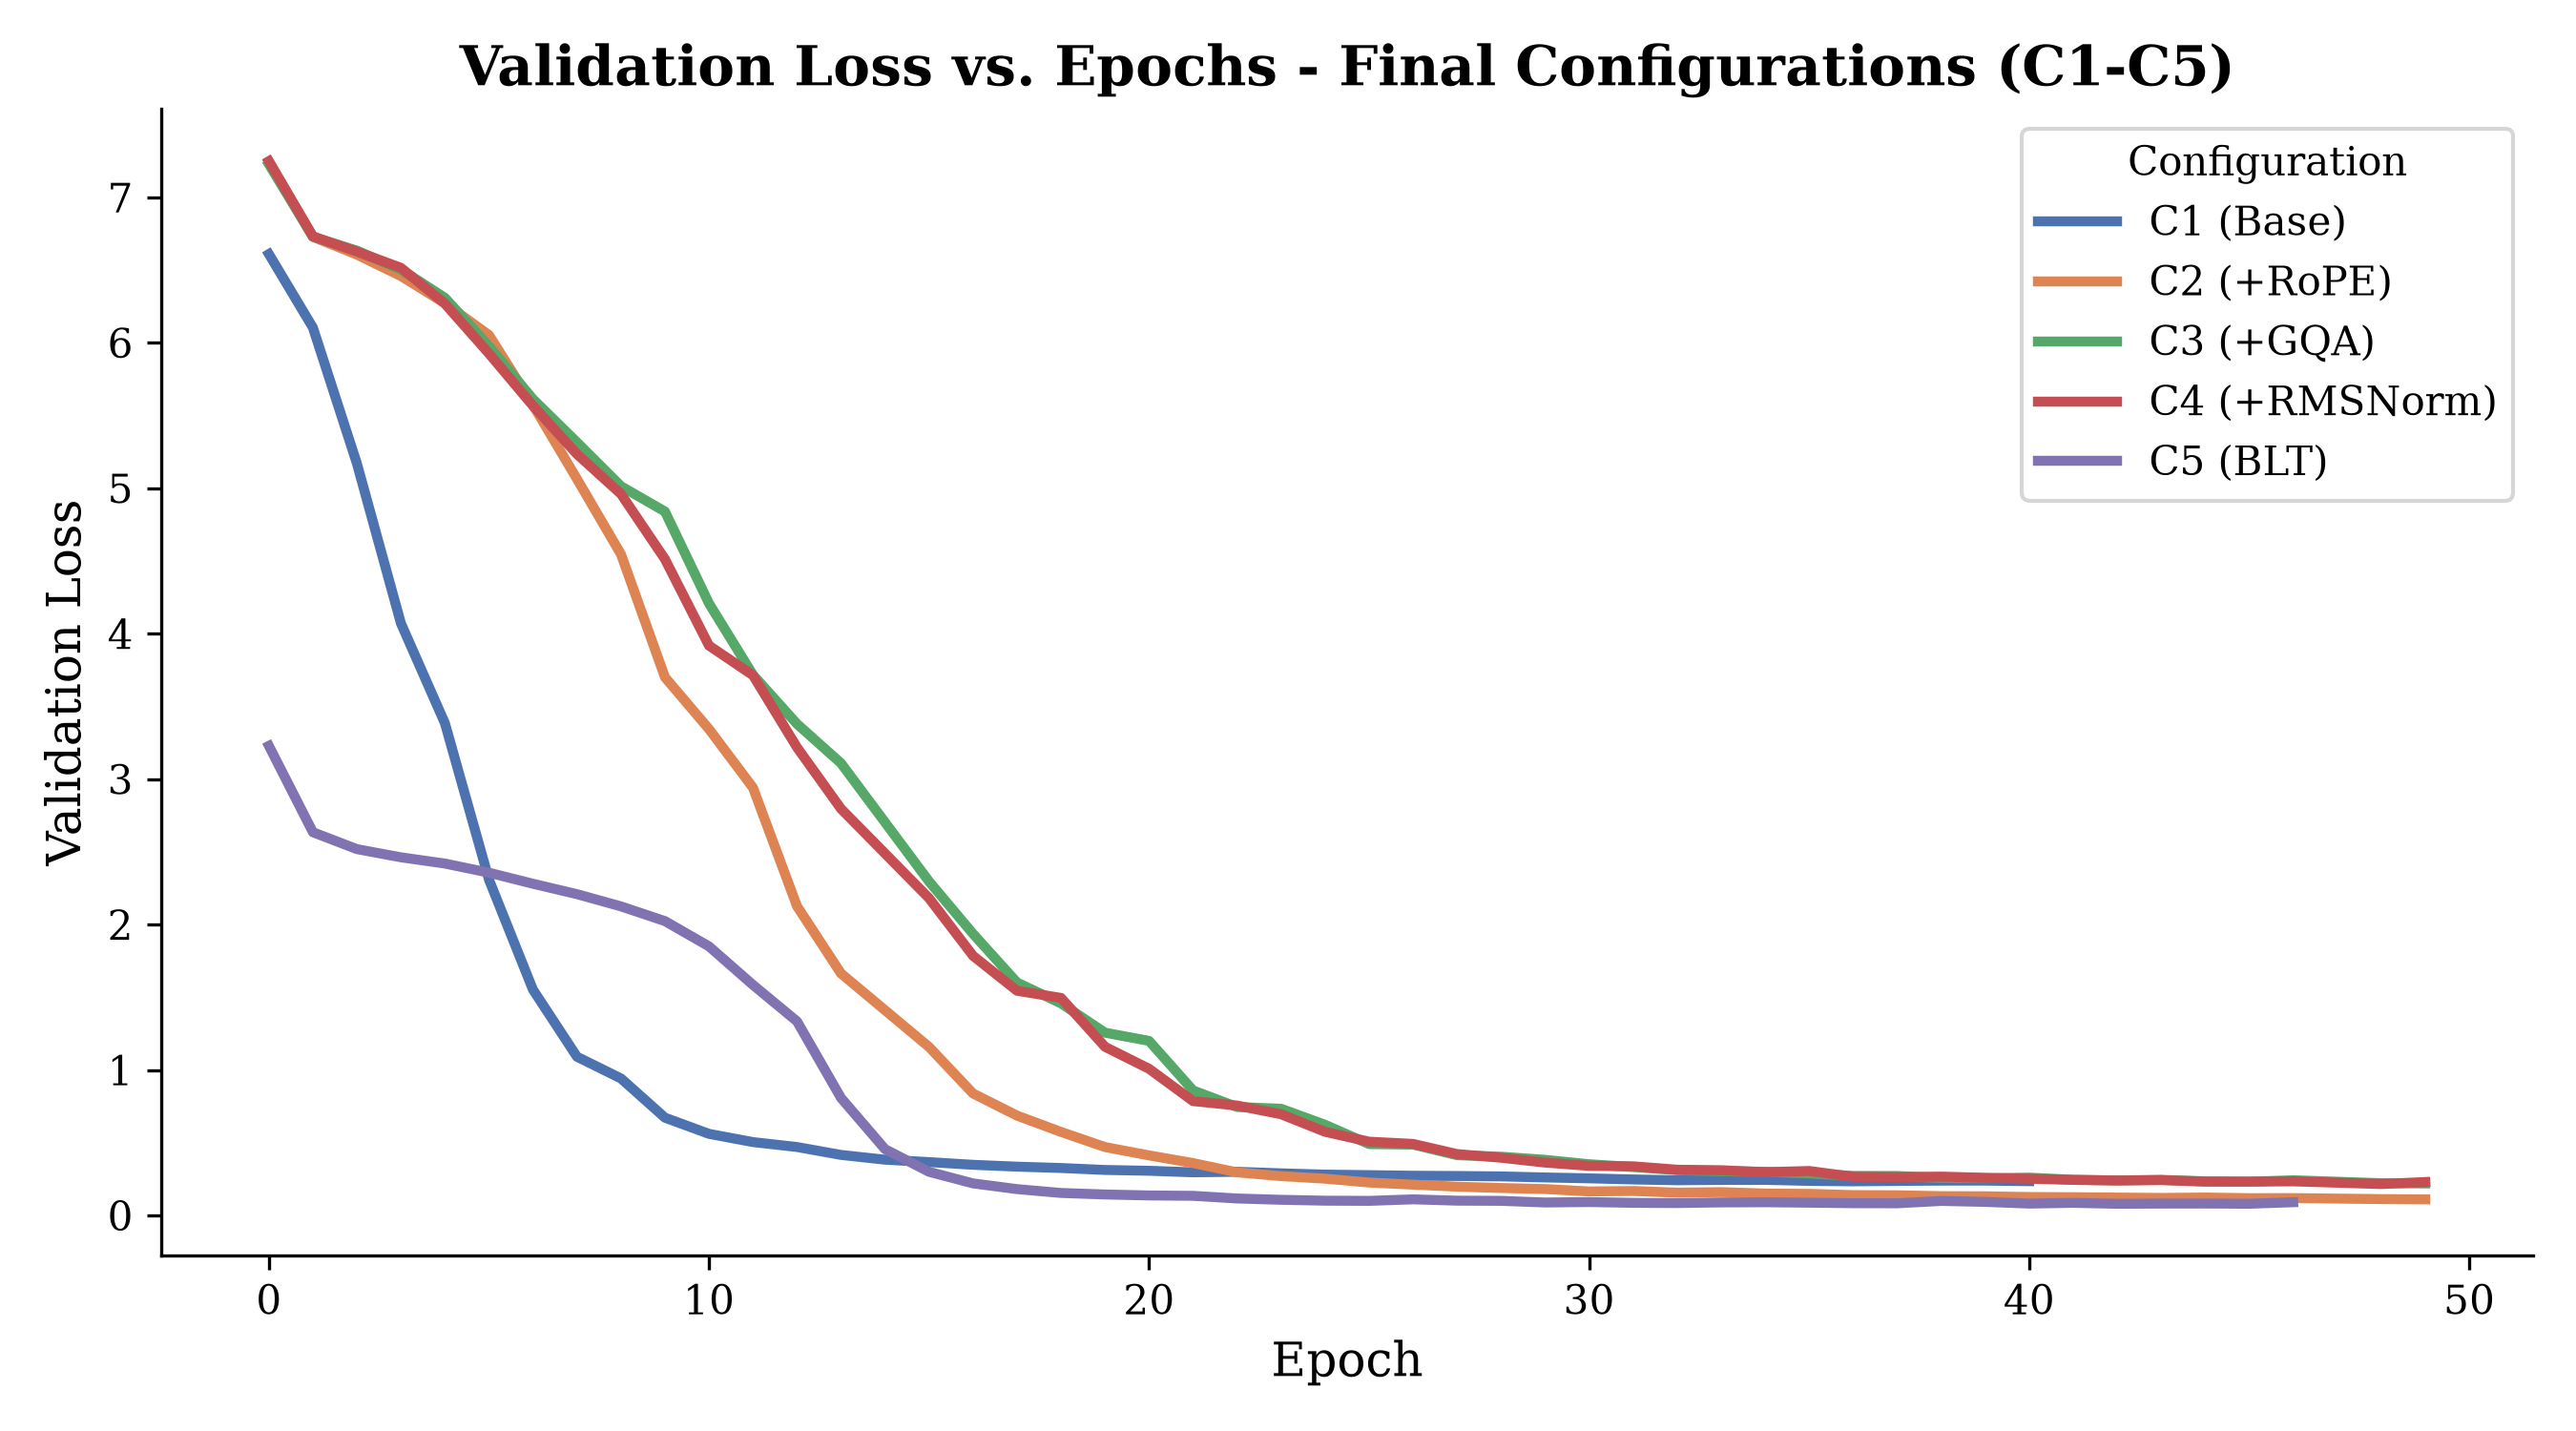
\includegraphics[width=0.75\linewidth]{outputs/val_loss_vs_epochs_final.png}
    \caption{Validation loss vs. epoch for the five final configurations. C5 reaches the lowest loss and stops early at epoch 46. C1 plateaus earliest (epoch 40) after a fast initial drop; C2-C4 continue improving past it and finish close to the full 50 epochs.}
    \label{fig:val_loss_final}
\end{figure}

\subsection{Component-by-Component Discussion}

With the corrected full-test-set evaluation, the ranking across every metric in Table~\ref{tab:results} is consistent: C5 $>$ C2 $>$ C4 $>$ C3 $>$ C1, best to worst. Every single-component change to the baseline (RoPE, GQA, RMSNorm) improves on plain C1, and C5's fully token-free design improves on all of them by a wide margin.

\textbf{C5 (fully token-free) is the clear winner.} C1 already represents the ciphertext at the byte level, so the remaining difference in C5 is removing BPE from the plaintext output too, and reading the ciphertext as a raw bit stream the model patches into bytes internally rather than a pre-grouped byte sequence. This lifts bit accuracy from 84.56\% (C1) to 99.95\%, and cuts mean Levenshtein distance from 2.83 to 0.06. Our reading: BPE on the plaintext \emph{output} introduces irregular subword boundaries on the side the model has to actually generate, which is where accuracy is measured, and even C1's byte-grouped cipher input still forces a fixed, externally-imposed patch size. C5 is also the smallest model (7.11M vs 13.69M params), since its vocabulary is fixed at 259 rather than the $\sim$5,000-token plaintext BPE vocabulary.

\textbf{C2 (RoPE) is the best of the tokenized models}, and a genuine surprise: bit accuracy rises to 91.50\%, Levenshtein falls to 1.74, and C2 has the best BLEU/ROUGE of any tokenized model. Our design rationale (\texttt{spec.md}) argued for \emph{absolute} positional encoding, since the cipher's decoding of a block depends on its absolute offset in the line; RoPE encodes relative position instead, yet clearly helps. One possible reconciliation: within a 64-character chunk, the actual training unit, relative and absolute offsets are highly correlated, so RoPE may capture the structure that matters locally just as well while optimizing slightly more easily under our fixed learning rate. A dedicated ablation varying chunk size would be needed to confirm this.

\textbf{C4 (RMSNorm) and C3 (GQA) both improve over C1, modestly and closely}: C4 (bit accuracy 87.64\%, Levenshtein 2.35) and C3 (87.40\%, 2.43) sit between C2 and C1 on every metric, without the structurally disruptive error pattern (high accuracy paired with high edit distance) we had originally attributed to C3 before this evaluation was corrected. \textbf{C1 is now the weakest tokenized model}, and part of why is likely training regime, not just architecture: as flagged in Section 3, single-GPU C1 converges to a worse validation loss than the original 4-GPU run and is first of C1-C4 to hit early stopping (epoch 40 vs.\ close to 50 for C2-C4), plausibly because the shared learning rate was tuned for a larger batch than any configuration actually uses. We would not claim sinusoidal absolute PE, standard MHA, and LayerNorm are simply worse in some fundamental sense; a fairer test would retune the learning rate per configuration.

%% ============================================================
\section{C5 vs. C1: Memory and Speed}

The assignment asks specifically for a memory and speed comparison between C5 and C1. We report the numbers as measured from WandB system metrics for the final runs, including where they complicate the usual byte-level-is-cheaper narrative.

\begin{figure}[H]
\centering
\begin{subfigure}[b]{0.48\linewidth}
    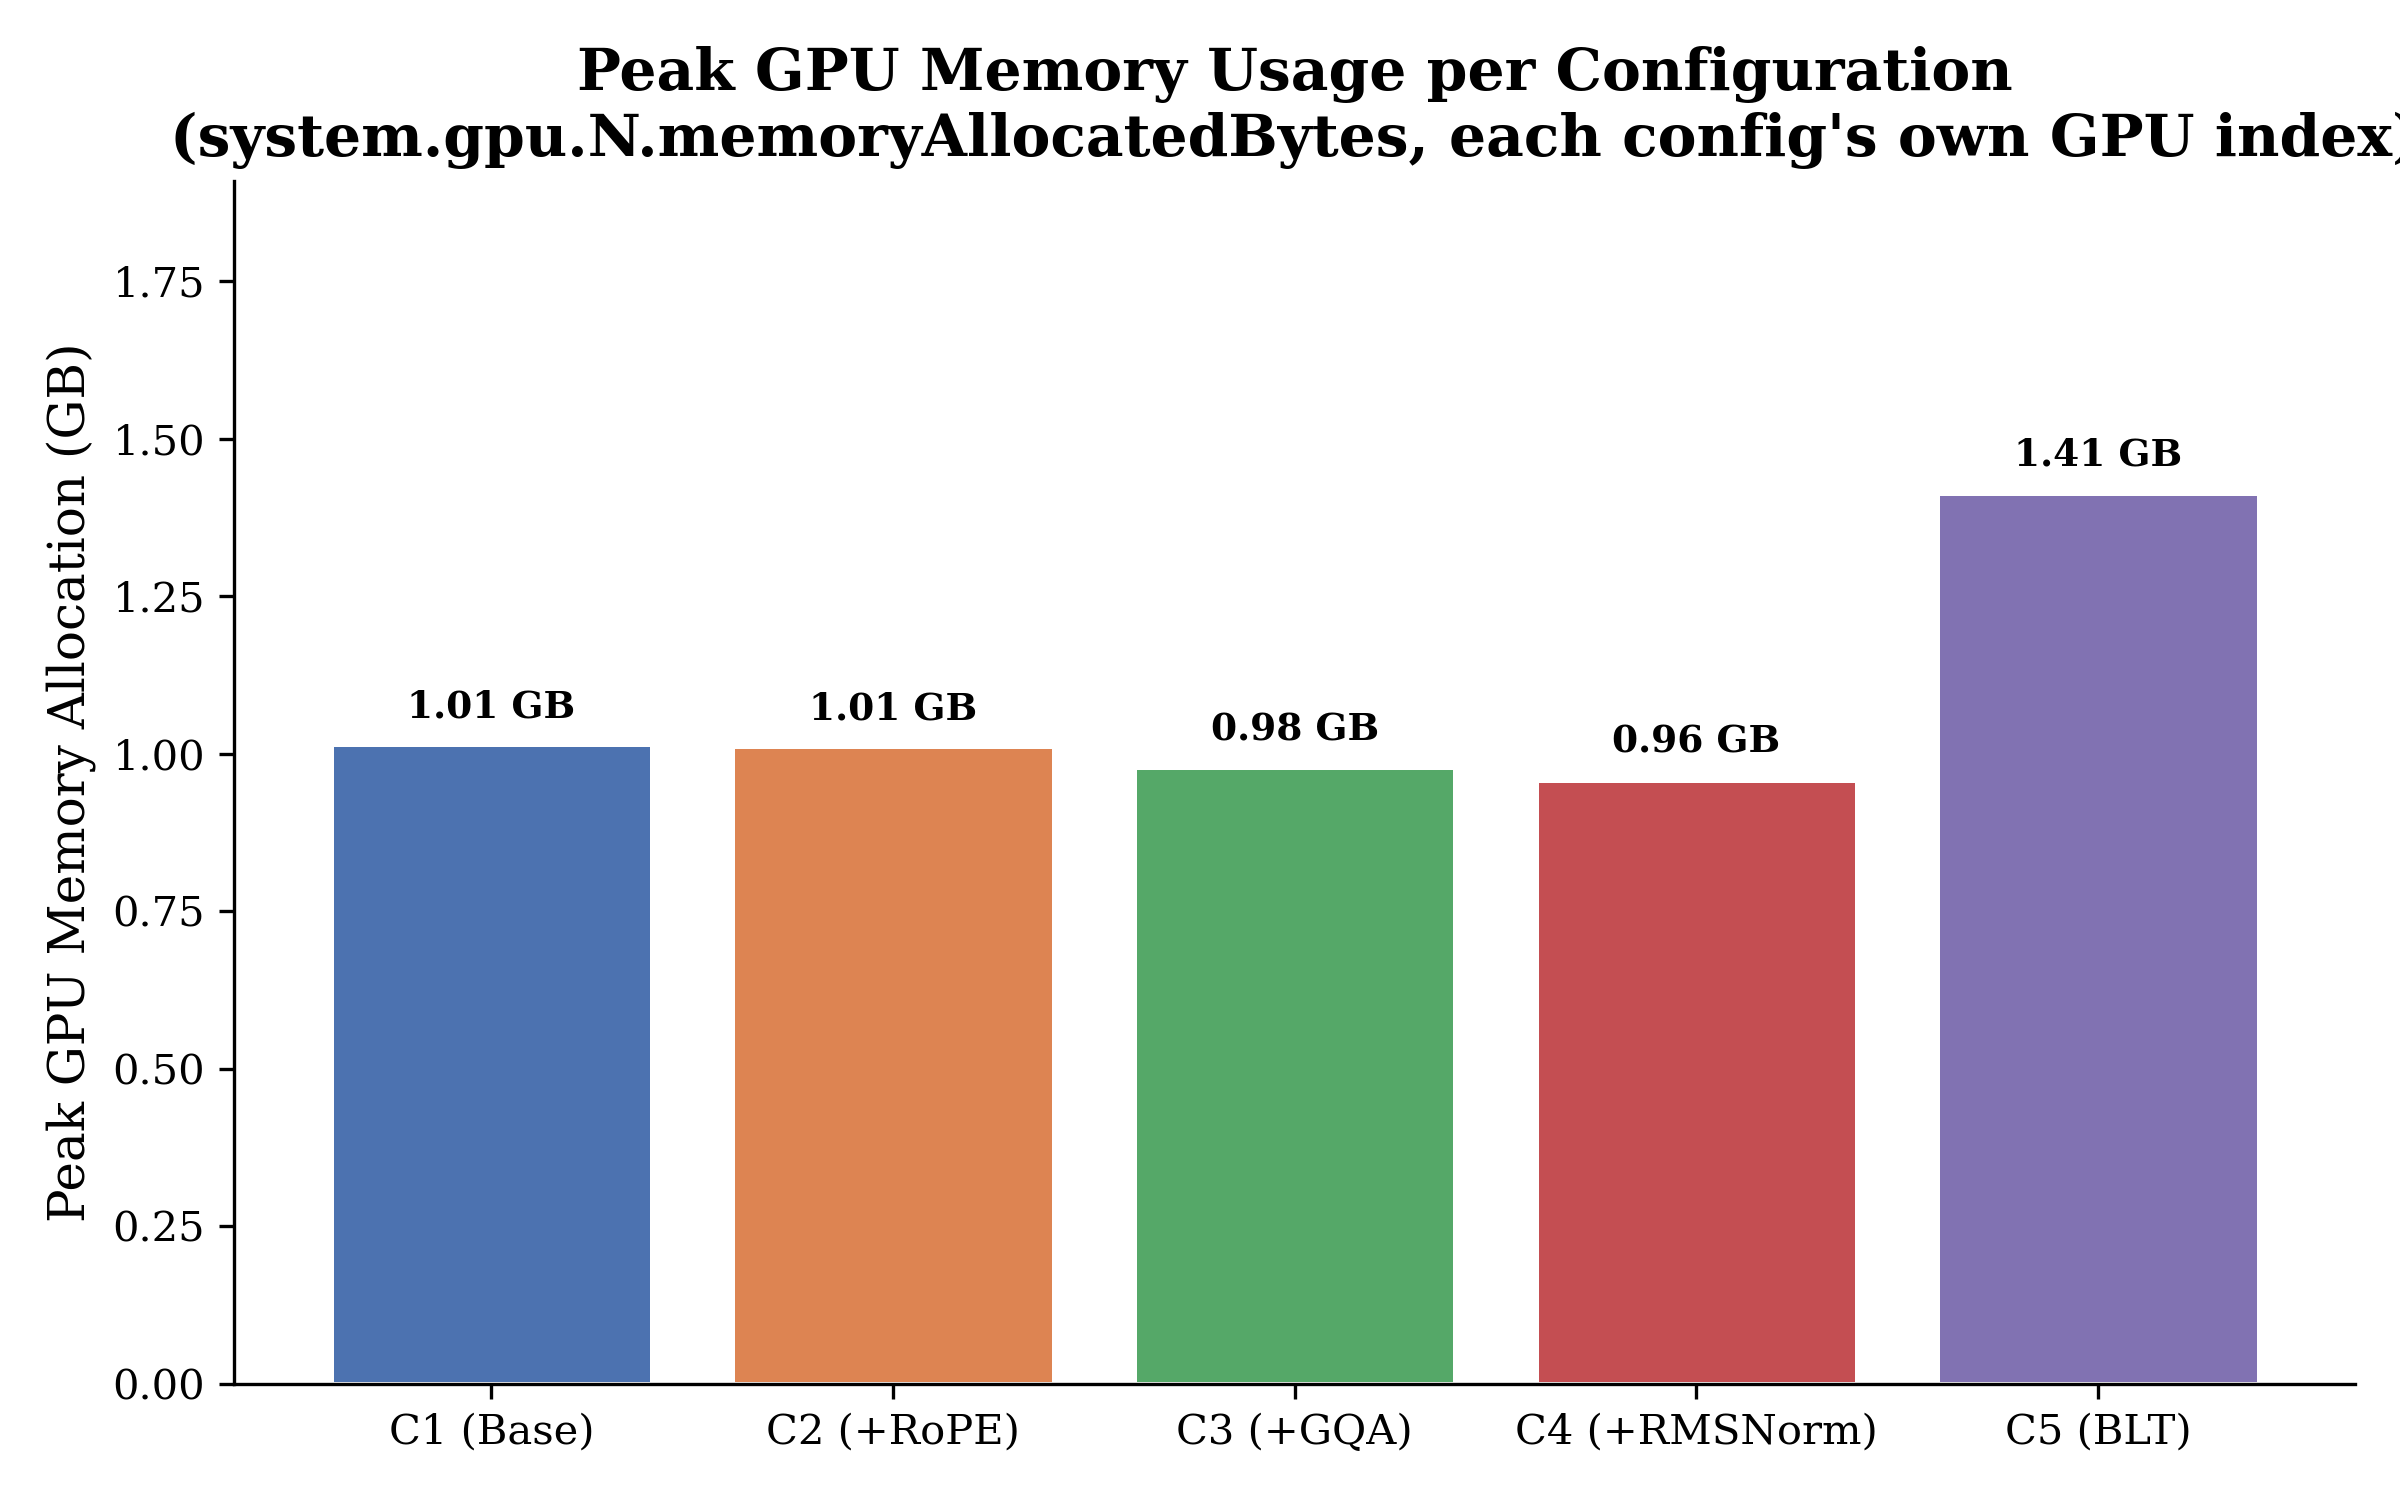
\includegraphics[width=\linewidth]{outputs/gpu_memory_comparison.png}
    \caption{Peak GPU memory per configuration.}
    \label{fig:gpu_mem}
\end{subfigure}
\hfill
\begin{subfigure}[b]{0.48\linewidth}
    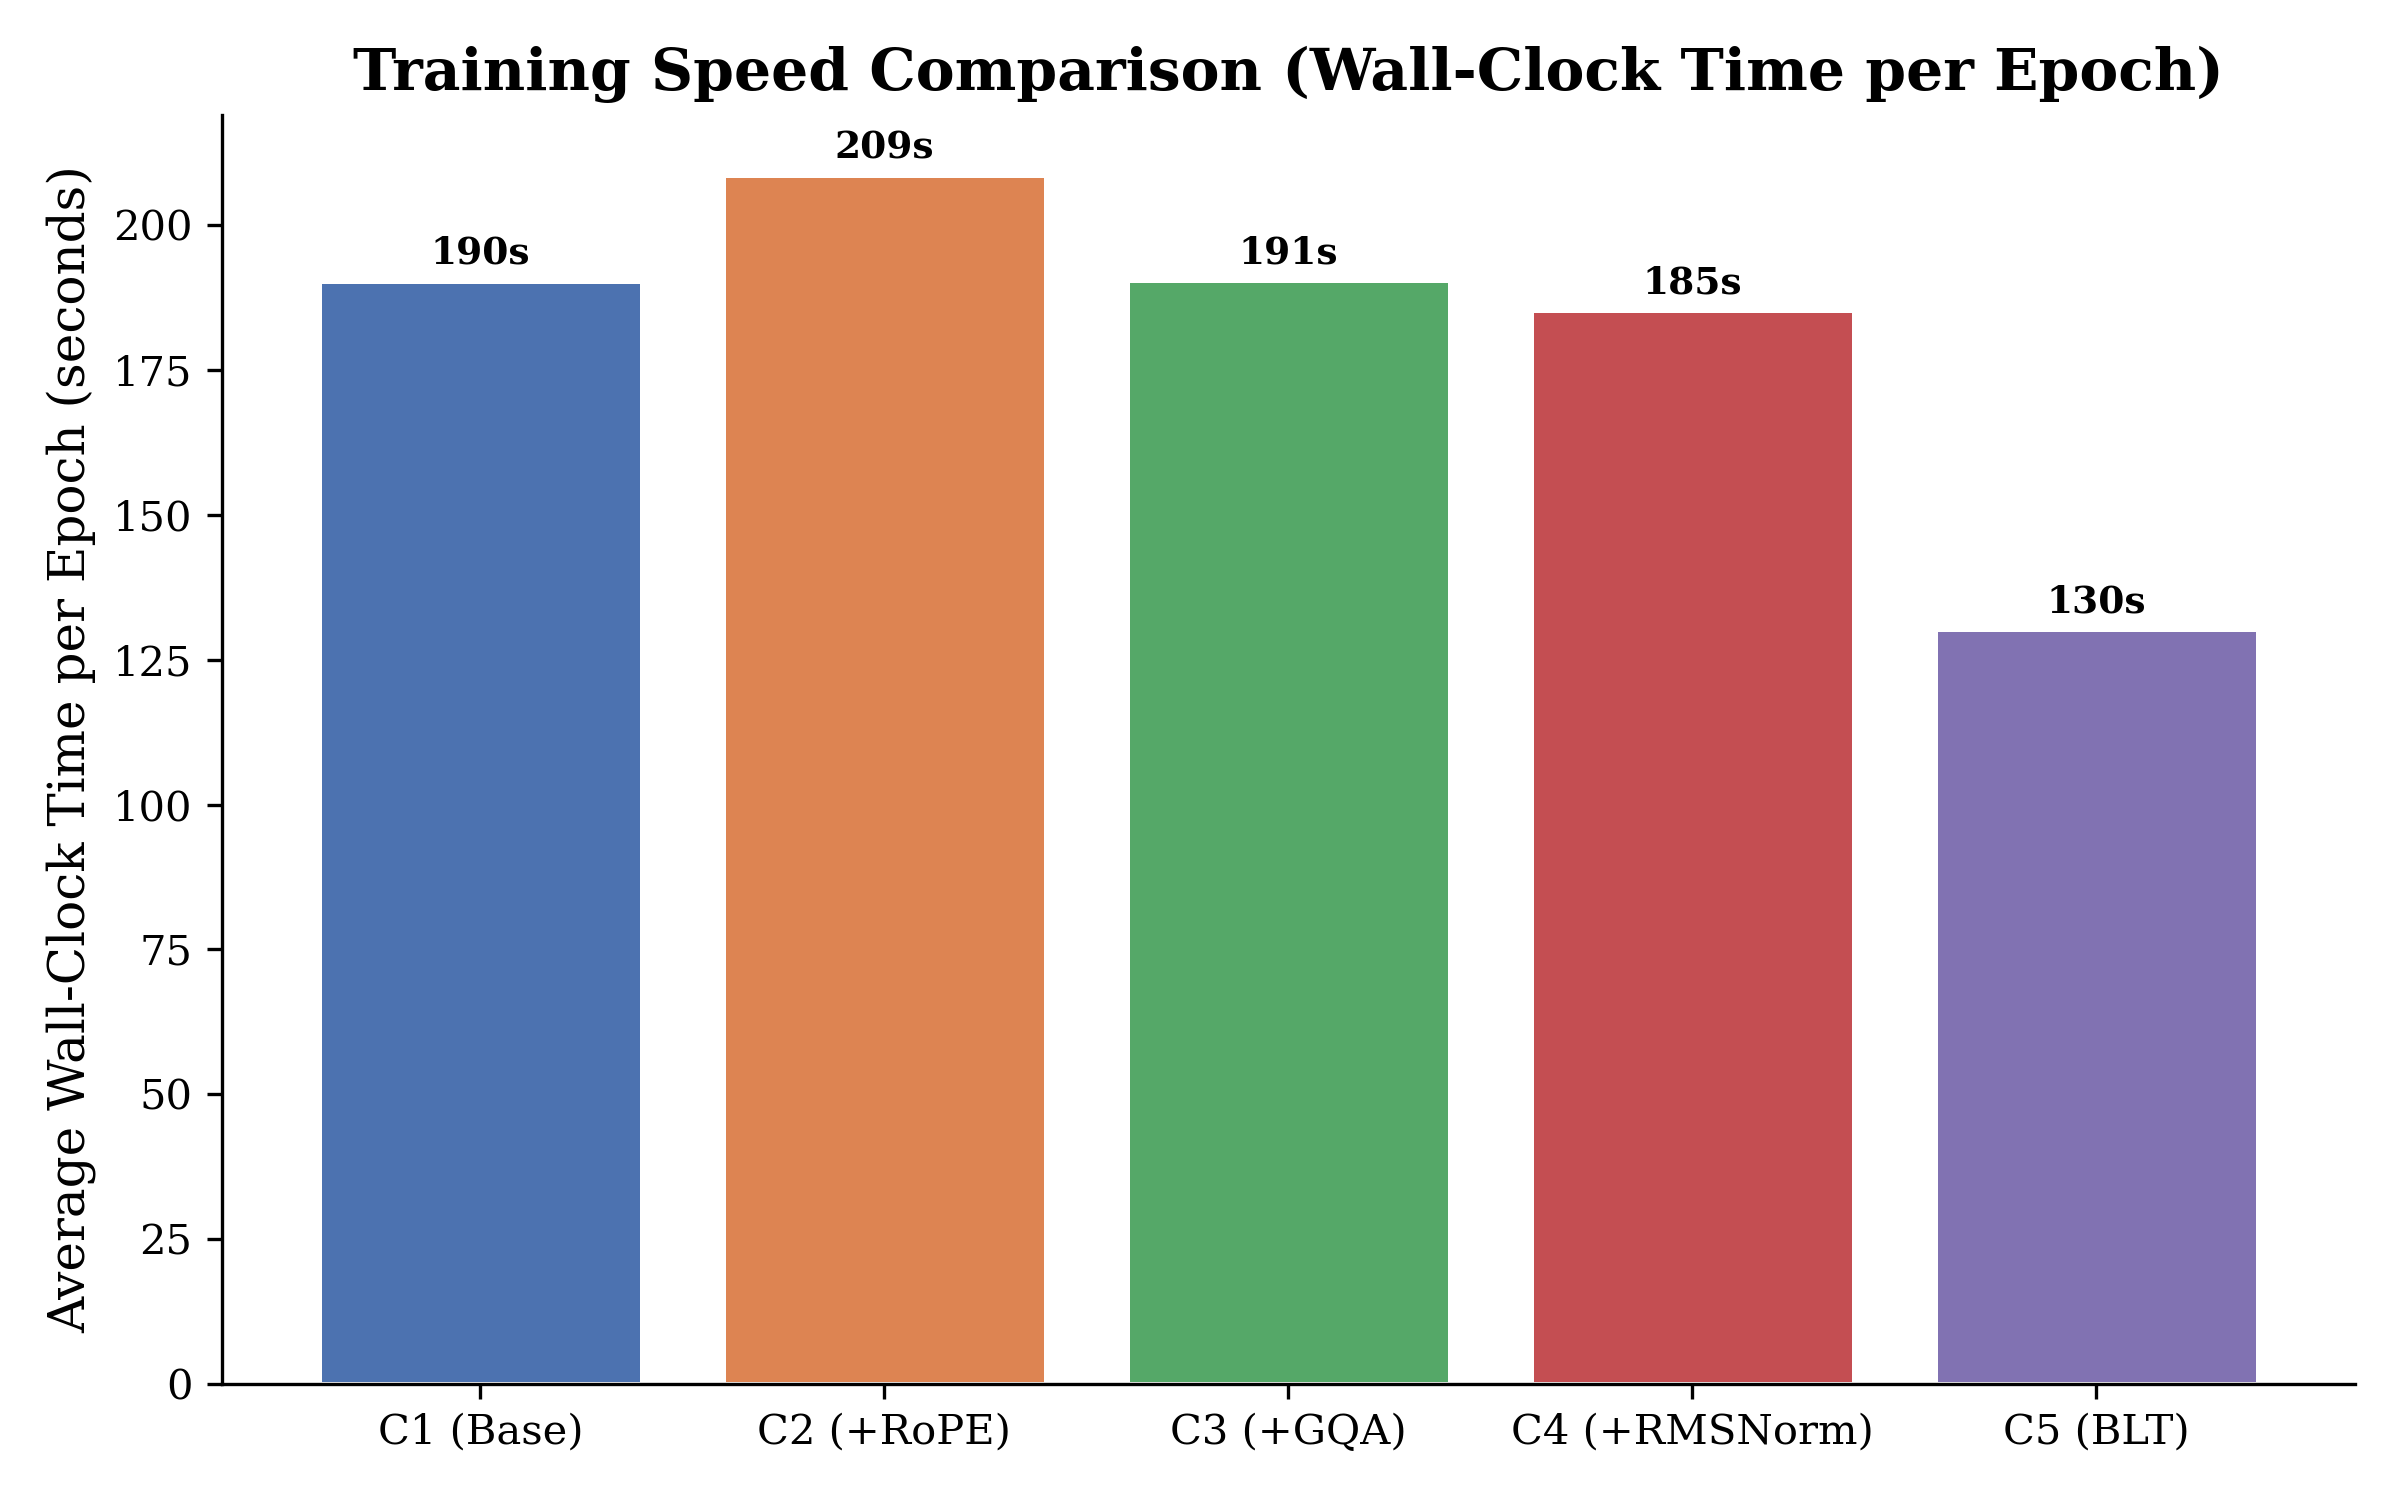
\includegraphics[width=\linewidth]{outputs/training_speed_comparison.png}
    \caption{Wall-clock time per epoch.}
    \label{fig:speed}
\end{subfigure}
\vspace{-4pt}
\caption{\small System metrics for all five final runs, each on a single RTX 2080 Ti (11 GB VRAM). C1's numbers are from run-C1-single-gpu-again, a repeat of the identical run on an otherwise-idle GPU (see the discussion below).}
\end{figure}

\textbf{Memory.} Our first attempt at this comparison reported an implausible $\approx$19.77 GB for C1, more than an 11 GB card can hold, next to $\approx$9.20 GB for C2-C5, and we initially explained the gap as another process sharing C1's GPU. Digging into it with a dedicated script (\texttt{src/check\_gpu\_stats.py}) turned up two real bugs, not one: first, the field we had been reading as "GPU memory in GB" (\texttt{system.gpu.N.memoryAllocated}) is actually a percentage of that GPU's total VRAM, not gigabytes; second, C2-C5 trained concurrently on the same four-GPU node, so each run's WandB system-metrics log also contains its three siblings' readings, since it polls every GPU on the machine, not just the one that run is using, and naively taking "the first GPU-memory column found" silently grabbed whichever sibling happened to sort first rather than the run's own GPU. Reading \texttt{system.gpu.N.memoryAllocatedBytes} from each config's actual confirmed GPU index gives a coherent picture: C1 and C2 are effectively identical ($\approx$1.01 GB each, as expected since RoPE, like C1's sinusoidal encoding, needs no extra learned parameters), C3 is slightly lower ($\approx$0.98 GB, consistent with GQA's smaller key/value projections), C4 is lowest ($\approx$0.96 GB, consistent with RMSNorm dropping the bias and mean-centering terms LayerNorm needs), and C5 is highest of all ($\approx$1.41 GB) despite having the fewest parameters (7.11M): its raw bit-stream input is roughly eight times longer than C1-C4's byte-grouped sequence, so the longer sequence's activation memory outweighs its smaller parameter count. We also reran C1 once more in isolation (run-C1-single-gpu-again) purely to double check, since its original run happened to share a GPU with another process; that rerun peaked at 1.01 GB (vs.\ 2.17 GB, not 19.77 GB, once the original run's raw figure is correctly read in GB), and its wall-clock speed (190.5 s/epoch) matches the original single-GPU run (193.7 s/epoch) closely, confirming training itself was never affected, only this one metric's reading.

\textbf{Speed.} With every configuration now trained on a single GPU, the picture is much cleaner than an earlier draft of this comparison, which mixed a 4-GPU C1 run in with four single-GPU runs and produced numbers that were not meaningfully comparable. C5 is fastest per epoch at 130.3 s; C1 (190.5 s) and C3 (190.6 s) are essentially tied, with C4 close behind (185.4 s); C2 is slowest at 208.6 s. All five train on the same 39,683 chunked examples per epoch, so C5's speed is architectural, not incidental: despite an almost 8x longer input sequence (raw bits vs. C1-C4's byte-grouped tokens) and extra local encoder/decoder layers, its much smaller 7.11M-parameter footprint and 259-token vocabulary more than offset that. C1-C4's more modest spread (185-209 s) is plausibly ordinary cluster variance rather than anything attributable to RoPE, GQA, or RMSNorm individually. Together with Section 5.1: on equal hardware, C5 is both more accurate than every tokenized model and the fastest to train per epoch, though not the cheapest in memory, since its much longer raw-bit-stream sequence costs more activation memory than its small parameter count saves. The byte-level architecture is a clear win on accuracy and speed, with memory the one axis where the tokenized models' shorter sequences still have an edge, a more nuanced story than a single "byte-level is cheaper" narrative, and visible only once the GPU-count mismatch in the original C1 run and the memory-metric bugs above were corrected.

%% ============================================================
\section{Qualitative Error Patterns}

We did not save per-example decoded predictions during these runs, so rather than construct illustrative sentence pairs, we note what Table~\ref{tab:results} implies: bit accuracy and Levenshtein distance now move together consistently across all five configurations (C5 best on both, then C2, C4, C3, C1), unlike the earlier 5-sample evaluation, which suggested some models had many small errors while others had few large ones. This suggests a model more accurate at the character level also tends to make more localized errors, rather than the two trading off. A side-by-side of decoded outputs, with prediction logging enabled, would sharpen this further.

%% ============================================================
\section{Conclusion}

The dataset analysis at the start of this project predicted the final results well: the cipher is an 8-bit, position-dependent encoding, and the configuration that respects that structure most directly, C5, produces by far the best reconstruction quality (99.95\% bit accuracy, 0.06 mean Levenshtein distance) with the fewest parameters and, on equal single-GPU hardware, the fastest training too, evaluated on the full 4,782-example test set. This was not obvious from the start: our earliest capacity sweep suggested a much larger model was needed, and only after tracing that back to a flawed cipher tokenizer did the shipped C1-C4 models shrink to \texttt{d\_model}=256 while still improving; fixing the representation mattered more than scaling the model. Among the tokenized models, every single-component change improved on plain C1 (RoPE most, RMSNorm and GQA more modestly), including the surprise of RoPE outperforming the absolute positional encoding our design rationale argued for, which we can only partly explain and some of which is plausibly a training-regime artifact: the shared learning rate was tuned for a larger effective batch than any final configuration actually trains under.

Three corrections shaped this report as much as the architecture results themselves. First, our test-set evaluation was originally restricted to 5 examples by a leftover debugging shortcut, caught because several metrics landed on suspiciously round fractions of 5; re-evaluating every checkpoint on the full test set reversed our earlier finding that RoPE and RMSNorm did not help and that GQA's accuracy came with unusually disruptive errors. Second, C1 was originally trained on 4 GPUs while C2-C5 trained on one, making the efficiency comparison in Section 6 meaningless until we retrained C1 to match. Third, our GPU memory readings were wrong in two compounding ways: we had been reading a WandB field that turned out to be a percentage of VRAM as if it were gigabytes, and since C2-C5 trained concurrently on a shared four-GPU node, naively picking "the first GPU-memory column" pulled in a sibling run's reading rather than each config's own; correcting both turned an implausible, seemingly architecture-defying result (C1 apparently using more memory than a full card holds) into a coherent one where every ablation's memory usage matches its design. All three are the kind of mistake that is easy to make and, we think, more useful to disclose than to quietly fix. A useful next step would be retuning the learning rate per configuration, and logging decoded predictions so a qualitative error analysis could be grounded in real examples rather than metric-level inference.

%% ============================================================
\section{Links}

\small
\textbf{WandB Project:} \url{https://wandb.ai/yash-more1224-international-institute-of-information-tec/anlp-assignment-1} \\
\textbf{WandB Runs:} run-C1-single-gpu, run-C2, run-C3, run-C4, run-C5 (final runs; train/val/test metrics and loss curves are from these five) plus run-C1-single-gpu-again (identical rerun of C1 in isolation, used only for the Section 6 memory/speed numbers; see the discussion there). All other runs, including the original 4-GPU run-C1, are exploratory. \\
\textbf{Hugging Face Checkpoints:} C1: \url{YOUR_HF_LINK_C1} \; C2: \url{YOUR_HF_LINK_C2} \; C3: \url{YOUR_HF_LINK_C3} \; C4: \url{YOUR_HF_LINK_C4} \; C5: \url{YOUR_HF_LINK_C5}
\normalsize

%% ============================================================
\vspace{3pt}
\hrule
\vspace{2pt}
\bibliographystyle{plainnat}
\begin{thebibliography}{9}

\bibitem{vaswani2017attention}
Vaswani, A., Shazeer, N., Parmar, N., Uszkoreit, J., Jones, L., Gomez, A. N., Kaiser, L., and Polosukhin, I. (2017).
\textit{Attention is all you need}.
NeurIPS 2017.

\bibitem{su2024roformer}
Su, J., Lu, Y., Pan, S., Murtadha, A., Wen, B., and Liu, Y. (2024).
\textit{RoFormer: Enhanced transformer with rotary position embedding}.
Neurocomputing, 568.

\bibitem{ainslie2023gqa}
Ainslie, J., Lee-Thorp, J., de Jong, M., Zewei, Y., Sanghai, S., and Xu, Y. (2023).
\textit{GQA: Training generalized multi-query transformer models from multi-head checkpoints}.
EMNLP 2023.

\bibitem{zhang2019rmsnorm}
Zhang, B. and Sennrich, R. (2019).
\textit{Root mean square layer normalization}.
NeurIPS 2019.

\bibitem{pagnoni2024blt}
Pagnoni, A., et al. (2024).
\textit{Byte latent transformer: Patches scale better than tokens}.
arXiv:2412.09871.

\end{thebibliography}

\end{document}
